\section{Test Case:User-defined Atmosphere Upwelling}
%====================================================

The user-defined atmosphere test case is sightly different for that of the built-in atmosphere in that the \texttt{TAPE5} uses defined surface emissivities and reflectivities, includes CFC profile information, and invokes the FFT scanning function.

\subsection{Double precision linux results}
%------------------------------------------
The double precision results for the linux system for the user-defined atmosphere test case
\begin{figure}[htp]
  \centering
  \qquad\sffamily\textbf{Verification Example: User-defined Atmosphere Upwelling}\\
  \qquad\sffamily\textbf{Red Hat linux platform; double precision}\\
  \qquad\textsf{LBLRTM v11.3 brightness temperature difference using a locally generated TAPE3}\\
  \includegraphics[bb=85 403 534 558,clip,scale=1.0]{graphics/run_example_user_defined_upwelling/dbl.eps}
  \qquad\textsf{LBLRTM v11.3 brightness temperature difference using AER TAPE3}\\
  \includegraphics[bb=85 226 534 381,clip,scale=1.0]{graphics/run_example_user_defined_upwelling/dbl.eps}
  \caption{User-defined Atmosphere Test: Comparison of the AER-supplied \texttt{TAPE27\_ex} output to the locally generated \texttt{TAPE27} output for the \textsl{double precision} version of LBLRTM v11.3 running on a Red Hat linux system. \mbox{\textbf{(a)} Using} a locally generated little-endian \texttt{TAPE3} spectroscopic datafile. \mbox{\textbf{(b)} Using} the AER-supplied little-endian \texttt{TAPE3} spectroscopic datafile.}
  \label{fig:run_example_user_defined_upwelling-dbl}
\end{figure}


\subsection{Double precision AIX results}
%-------------------------------------------
\begin{figure}[htp]
  \centering
  \qquad\sffamily\textbf{Verification Example: User-defined Atmosphere Upwelling}\\
  \qquad\sffamily\textbf{IBM AIX platform; double precision}\\
  \qquad\textsf{LBLRTM v11.3 brightness temperature difference using a locally generated TAPE3}\\
  \includegraphics[bb=85 403 534 558,clip,scale=1.0]{graphics/run_example_user_defined_upwelling/dbl_ibm.eps}
  \qquad\textsf{LBLRTM v11.3 brightness temperature difference using AER TAPE3}\\
  \includegraphics[bb=85 226 534 381,clip,scale=1.0]{graphics/run_example_user_defined_upwelling/dbl_ibm.eps}
  \caption{User-defined Atmosphere Test: Comparison of the AER-supplied \texttt{TAPE27\_ex} output to the locally generated \texttt{TAPE27} output for the \textsl{double precision} version of LBLRTM v11.3 running on an IBM AIX system. \mbox{\textbf{(a)} Using} a locally generated big-endian \texttt{TAPE3} spectroscopic datafile. \mbox{\textbf{(b)} Using} the AER-supplied big-endian \texttt{TAPE3} spectroscopic datafile.}
  \label{fig:run_example_user_defined_upwelling-dbl_ibm}
\end{figure}


\subsection{Single precision run results}
%----------------------------------------

\begin{figure}[htp]
  \centering
  \qquad\sffamily\textbf{Verification Example: User-defined Atmosphere Upwelling}\\
  \qquad\sffamily\textbf{Red Hat linux platform; single precision}\\
  \qquad\textsf{LBLRTM v11.3 brightness temperature difference using a locally generated TAPE3}\\
  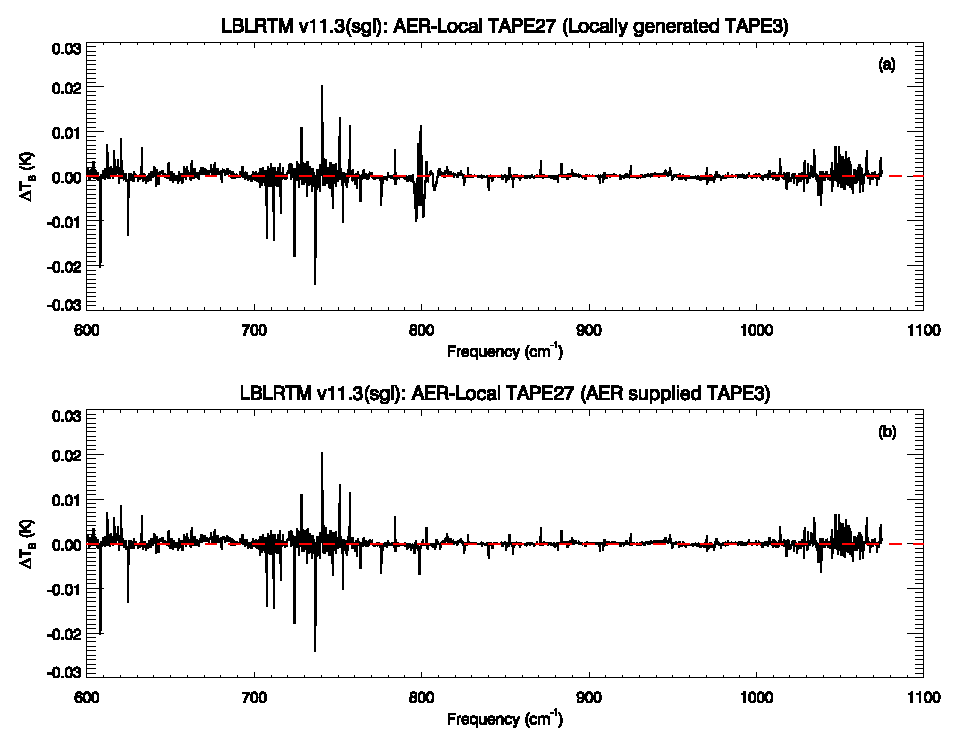
\includegraphics[bb=85 403 534 558,clip,scale=1.0]{graphics/run_example_user_defined_upwelling/sgl.eps}
  \qquad\textsf{LBLRTM v11.3 brightness temperature difference using AER TAPE3}\\
  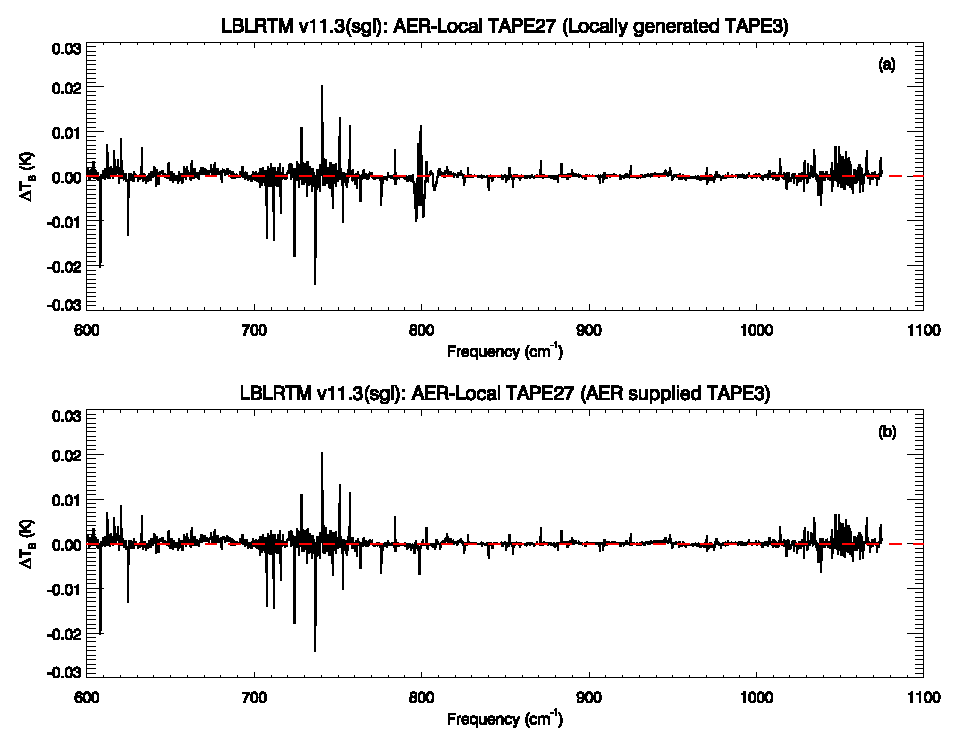
\includegraphics[bb=85 226 534 381,clip,scale=1.0]{graphics/run_example_user_defined_upwelling/sgl.eps}
  \caption{User-defined Atmosphere Test: Comparison of the AER-supplied \texttt{TAPE27\_ex} output to the locally generated \texttt{TAPE27} output for the \textsl{single precision} version of LBLRTM v11.3 running on a Red Hat linux system. \mbox{\textbf{(a)} Using} a locally generated little-endian \texttt{TAPE3} spectroscopic datafile. \mbox{\textbf{(b)} Using} the AER-supplied little-endian \texttt{TAPE3} spectroscopic datafile.}
  \label{fig:run_example_user_defined_upwelling-sgl}
\end{figure}

\begin{figure}[htp]
  \centering
  \qquad\sffamily\textbf{Verification Example: User-defined Atmosphere Upwelling}\\
  \qquad\sffamily\textbf{IBM AIX platform; single precision}\\
  \qquad\textsf{LBLRTM v11.3 brightness temperature difference using a locally generated TAPE3}\\
  \includegraphics[bb=85 403 534 558,clip,scale=1.0]{graphics/run_example_user_defined_upwelling/sgl_ibm.eps}
  \qquad\textsf{LBLRTM v11.3 brightness temperature difference using AER TAPE3}\\
  \includegraphics[bb=85 226 534 381,clip,scale=1.0]{graphics/run_example_user_defined_upwelling/sgl_ibm.eps}
  \caption{User-defined Atmosphere Test: Comparison of the AER-supplied \texttt{TAPE27\_ex} output to the locally generated \texttt{TAPE27} output for the \textsl{single precision} version of LBLRTM v11.3 running on an IBM AIX system. \mbox{\textbf{(a)} Using} a locally generated big-endian \texttt{TAPE3} spectroscopic datafile. \mbox{\textbf{(b)} Using} the AER-supplied big-endian \texttt{TAPE3} spectroscopic datafile.}
  \label{fig:run_example_user_defined_upwelling-sgl_ibm}
\end{figure}

